The development of a sprint is composed by multiple phases, as shown in figure \ref{fig:reply:workflow}.

\begin{figure}
    \centering
    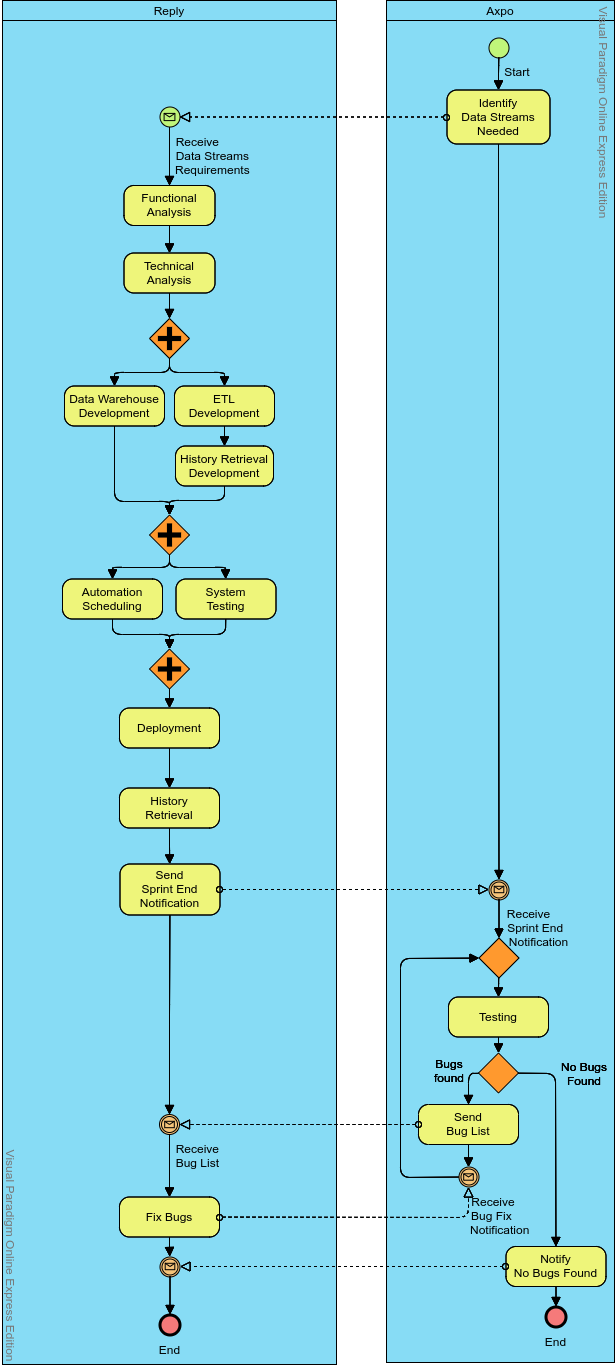
\includegraphics[width=\textwidth,height=\textheight,keepaspectratio]{res/reply_workflow.png}
    \caption{Workflow used by Reply.}
    \label{fig:reply:workflow}
\end{figure}

\paragraph{Functional analysis}
    % ora, sito, link
The goal of functional analysis is to get a high-level understanding of the data needed for the sprint.

This role requires to analyze each provider, learning which data streams to download, where to download them from and how often the data needs to be downloaded.

The result of this work is an Excel file, containing information such as:
\begin{itemize}
    \item A detailed list of each data stream required for each provider.
    \item The update frequency of each data stream.
    \item A download schedule for each data stream.
    \item A download URL per data stream.
\end{itemize}

\paragraph{Technical analysis} 
   The next step is to take these high-level information and provide some very detailed instructions on how to download the data.

These information are very technical in nature, such as which method (for example, an \textit{HTTP GET} call) or parameters need to be used to download a specific datum, as well as which operations must be applied to transforming the downloaded data properly.

These information are then passed on to the developers, who write the actual implementation.
\paragraph{ETL development}
    Developers receive the low-level specifications written during the technical analysis and implement the actual ETL process.

This process, implemented on Azure Databricks, needs to retrieve data from multiple providers using different techniques.
Several cleaning and normalization operations are then applied on the data downloaded.
Finally, the results are loaded into the Data Warehouse.
\paragraph{History retrieval development}
    The ETL procedure downloads data for a single day\footnote{
    To be more precise, the process downloads data for a single time unit, i.e,. the scheduled download interval for a given stream.
    Most streams are downloaded daily, but some have a different download frequency (varying from hourly to two or three times a day).
} but, during the Data Warehouse initialization, it is necessary to download data up to a few years before.

This process creates a wrapper for the ETL procedure, calling it several times, each time downloading data for a different day.
The procedure is iterative, meaning that a single day will be extracted, transformed and loaded before processing the next day.

Days are downloaded backwards.
This allows to handle errors, such as file structure changes, more efficiently, since they will not affect any file downloaded up to that point.

\paragraph{Data Warehouse design} 
    The ETL process needs to load the transformed data on the Data Warehouse.

Its design is done in parallel, by a different team, with the ETL process.
The design process is responsible for the following actions:
\begin{itemize}
    \item Creating some tables onto which the ETL process will load the data \textit{as-is}.
    
    \item Creating a procedure for performing some operations on the data, such as remapping or adding constants.
    
    \item Loading the data onto the actual end-user tables, as well as checking if the data actually needs to be loaded.
    \begin{itemize}
        \item Some values may already be present if the ETL process for a given time range is executed multiple times, for example due to errors.
    \end{itemize}
\end{itemize}

\paragraph{Automation scheduling}
    Each website provides new data at regular intervals.
It is thus necessary to execute the ETL process each time the provider has new data.

During the functional analysis, each provider has been marked with its update frequency.
This process schedules, for each flow, when the ETL process will be executed, ranging from once a month to multiple times a day.

Since it is necessary to download multiple data streams from each provider, Reply decided to schedule a single job per provider which executes all jobs required for that provider.

A secondary function of the scheduling process is to pause the whole Data Warehouse at night, since it is not going to be used, to reduce cloud maintenance costs.

\paragraph{System testing}
    Functional and technical analysts must also make sure that the whole ETL process is working as intended and that the data downloaded into the Data Warehouse is identical to that present in the original websites.

These tests are done by both analysts together by hand.
They manually check some data samples from the data warehouse and compare them with the same values in the websites.

This testing phase is focused mainly on the following aspects:
\subpar{Number of rows}
    Testers manually assert that the number of imported values in the Data Warehouse (i.e. table rows) is the same than those available on the website.
    
    As such, they can be sure the ETL process didn't lose any values.

\subpar{Conversion errors}
    Testers check columns on which conversion operations have been applied, to make sure the process completed successfully.
    
    These checks for example assert that decimal numbers have been correctly interpreted, dates have been properly remapped and that each column contains the right kind of data.
    
\subpar{Sample checking}
    Lastly, testers take same sample rows and compare all their values with the data available on the website.
    
    If all the values are identical, then it's likely the ETL process is working properly and that all the other values will be correct too.


\paragraph{Deployment to production environment}
    The last step is to deploy the whole structure to the production environment.

The deployment is done by exporting all the scripts used (for both the ETL process and the Data Warehouse configuration) and re-importing them into the new environment.
All scripts are then executed, in order to:
\begin{enumerate}
    \item Initialize (or modify, if they already exist) all tables and procedures in the Data Warehouse.
    
    \item Download the first set of data (typically up to a few years before).
\end{enumerate}

This phase is the most delicate, since this environment is used for production, so it is imperative that the deployment must not cause any errors.

Particular attention must also be paid to the update of existing structures.
For example, if a table structure has to be changed, it is not possible to simply drop and recreate it, since all data would be lost.
It is then necessary to compute the difference between the two versions, and to update as needed.
\paragraph{History retrieval}
    After deployment, the Data Warehouse is empty and needs to be initialized.

Initialization is done by invoking the apposite procedures previously developed.

The process takes a long time to execute, usually a few hours per provider, but only needs to be executed once.

% However, this phase has been proven to be vulnerable to unexpected errors.
% For example, some providers have changed file structure a few years ago, which broke the history retrieval process for those data.

% As a consequence, Reply decided to anticipate this phase during development, encountering and solving these errors before the deployment deadline.
% After deployment this process will then be very likely to succeed without errors.
\paragraph{User Acceptance Test}
    The system is finally tested by the various Axpo departments users.

If they notice any problem, they notify Reply, which develops and applies the appropriate fixes.

Some are not specific or predefined, but rather mainly consist of the users trying to use the Data Warehouse for their actual needs, such as running their algorithms.

Other tests are more systematic, such as the ones described in chapter \ref{section:tests:data}.
